% \begin{filecontents}{\jobname.bib}
% @book{Dumke2001,
%     Author = {Dumke},
%     Publisher = {Vieweg},
%     Title = {Software-Engineering},
%     Year = {2001},
%     ISBN = {3-528-25355-X}}
% @book{Balzert1998,
%     Author = {BALZERT, H.},
%     Publisher = {Spektrum Akademischer Verlag},
%     Title = {Lehrbuch der Software-Technik, Band 2: Software-Management, Software-Qualit"atssicherung},
%     Year = {2001},
%     ADDRESS = {Heidelberg; Berlin; Oxford},
%     ISBN = {978-3827400659}}
% \end{filecontents}

% DUMKE (2001): Software-Engineering, Vieweg, ISBN 3-528-25355-X

%%%%%%%%%%%%%%%%%%%%%%%%%%%%%%%%%%%%%%%%%%%%%%%%%%%%%%%%%%%%%%%%%%%%%
% LaTeX Template: Softwaretechnik SS 2017
%
% Date: April 2017
%
%%%%%%%%%%%%%%%%%%%%%%%%%%%%%%%%%%%%%%%%%%%%%%%%%%%%%%%%%%%%%%%%%%%%%%

\documentclass[12pt]{article}
\usepackage[a4paper]{geometry}
\usepackage{framed}
\usepackage[myheadings]{fullpage}
\usepackage{fancyhdr}
\usepackage{lastpage}
\usepackage{graphicx, wrapfig, subcaption, setspace, booktabs}
% \usepackage{movie15}
\usepackage[T1]{fontenc}
\usepackage[font=small, labelfont=bf]{caption}
\usepackage[protrusion=true, expansion=true]{microtype}
\usepackage[ngerman]{babel}
\usepackage[ngerman]{translator}
\usepackage{sectsty}
\usepackage{url, lipsum}
\usepackage[parfill]{parskip}
\usepackage{csquotes}
\usepackage[hidelinks]{hyperref}
\usepackage[acronym]{glossaries}

% \usepackage[utf8]{inputenc}

% \bibliographystyle{numeric}

% \usepackage[style=authoryear,backref=tr"u]{biblatex}
\usepackage[sorting=none,backref=true, backend=biber]{biblatex}
\addbibresource{\jobname.bib}
% \usepackage[numbers,round]{natbib}
% \AtEveryCitekey{\clearfield{url}\clearfield{doi}\clearfield{isbn}\clearfield{issn}}


\usepackage[export]{adjustbox}
\usepackage{multicol}
\usepackage{tikz}
\usepackage{float}


\makeglossaries
\glstoctrue



%-------------------------------------------------------------------------------
% Commands
%-------------------------------------------------------------------------------
\newcommand{\HRule}[1]{\rule{\linewidth}{#1}}
\input{../env}
%-------------------------------------------------------------------------------
% HEADER & FOOTER
%-------------------------------------------------------------------------------
\pagestyle{fancy}
\fancyhf{}
\setlength\headheight{15pt}
\fancyhead[L]{\newCommandName}
\fancyhead[R]{\newCommandUniversity}
\fancyfoot[R]{Seite \thepage\ von \pageref{LastPage}}

%-------------------------------------------------------------------------------
% TITLE PAGE
%-------------------------------------------------------------------------------
\begin{document}
\hypersetup{
    % colorlinks,
    citecolor=black,
    filecolor=black,
    linkcolor=black,
    urlcolor=black
}


\title{ \normalsize
		\HRule{0.5pt} \\
		\LARGE \textbf{\uppercase{\newCommandDiscipline}} \\
    \smallbreak
		\small\textbf{{\newCommandTerm}}\\
		\HRule{2pt} \\ [0.5cm]
		\normalsize \today \vspace*{10\baselineskip}}

\date{}

\author{
		\newCommandName \\
		\newCommandMatriculationNumber \\
		\newCommandUniversity \\
		\newCommandFaculty
}

% \pagenumbering{gobble}

\maketitle
\thispagestyle{empty}

\newpage


\tableofcontents
\listoffigures
\newpage



%-------------------------------------------------------------------------------
% Section title formatting
\sectionfont{\scshape}
%-------------------------------------------------------------------------------

%-------------------------------------------------------------------------------
% BODY
%-------------------------------------------------------------------------------

\section{SWT - Einf"uhrung in die Softwaretechnik}

%-------------------------------------------------------------------------------
% #1
%-------------------------------------------------------------------------------

\newglossaryentry{st}{type=\acronymtype, name={ST}, description={Softwaretechnik}}
\newglossaryentry{ieee}{type=\acronymtype, name={IEEE}, description={Institute of Electrical and Electronics Engineers}}
\newglossaryentry{cmm}{name=CMM, description={Capability Maturity Model}}
\newglossaryentry{pmmm}{name=PMMM, description={Project Management Maturity Model}}

\subsection{"Ubung SWT-01}
\subsubsection*{Aufgabe:}

\begin{framed}
\textbf{Softwaretechnik allgemein}
\smallbreak
Was ist Softwaretechnik? Was wird da gelehrt? Worum geht es?
\\
Was antworten Sie?
\bigbreak
\small Bearbeitungszeit: 10 Minuten
\end{framed}
\bigbreak
\bigbreak
\subsubsection*{L"osung:}

\textbf{Der \gls{ieee}-Standard 610-1990 definiert Softwaretechnik als:}


\begin{center}
% \enquote{(1) The application of a \textbf{systematic}, \textbf{disciplined}, \textbf{quantifiable} approach to the development, operation, and maintenance of software; that is, the application of engineering to software. (2) The study of approaches as in (1)}
\enquote{The application of a  systematic\footnote{\label{foot:1}systematic - having, showing, or involving a system, method, or plan}, disciplined\footnote{\label{foot:2}disciplined - having or exhibiting discipline; rigorous}, quantifiable\footnote{\label{foot:3}quantifiable - to determine, indicate, or express the quantity of} approach to the development, operation, and maintenance of software; that is, the application of engineering to software.}
\end{center}

\bigbreak
\bigbreak

Aus dieser Definition k"onnen folgende Merkmale der \gls{st} benannt werden:
\bigbreak
\begin{itemize}
\item \gls{st} umfasst Methoden, Techniken und Instrumente zur Erstellung von auf Maschinen lauff"ahigen Programmen (Software).
\item Ziel von \gls{st} ist die Vermeidung von Fehlern, Reduktion von Aufw"anden und Erh"ohung des Kundennutzens von Software.
\item \gls{st} beinhaltet das Management von Entwicklungsprojekten f"ur Software.
\item \gls{st} umfasst die Inbetriebnahme, den Betrieb und die Wartung von Software.
\item Hierzu beschreibt \gls{st} bew"ahrte Vorgehensweisen in Modellen (Vorgehensmodelle) und definiert Qualit"atsstufen f"ur den Software-Entwicklungsprozess (\gls{cmm}, \gls{pmmm}).
\end{itemize}

\newpage

Dumke(2001)\supercite{Dumke2001} nimmt eine Einteilung in f"unf Kategorien vor:
\bigbreak
\begin{itemize}
\item \textbf{Methoden (development methods)}: \smallbreak Richtlinien, Strategien, und Technologien f"ur eine systematische, d. h. phasen- oder schrittweise Entwicklung von Software

\item \textbf{Werkzeuge (tools)}: \smallbreak rechnergest"utzte Hilfsmittel zur Software-Entwicklung und -Anwendung

\item \textbf{Ma"ssysteme (set of measurements)}: \smallbreak Menge von Software-Ma"sen zur Bewertung und Messung der Eigenschaften der zu entwickelnden Software hinsichtlich Eignung, Qualit"at und speziell des Leistungsverhaltens

\item \textbf{Standards (standards)}: \smallbreak Menge von Richtlinien f"ur die einheitliche und abgestimmte Form der Software-Entwicklung und des zu entwickelnden Software-Systems

\item \textbf{Erfahrungen (experiences)}: \smallbreak (quantifizierte) Kenntnisse "uber die Entwicklung der Software sowie das Entwicklungsergebnis selbst hinsichtlich des Einsatzes, der Qualit"at und des Nutzens (als Ingenieurwissen)
\end{itemize}


%-------------------------------------------------------------------------------
% #2
%-------------------------------------------------------------------------------
\newtheorem{defi}{Definition:}
\newpage
\subsection{"Ubung SWT-02}
\subsubsection*{Aufgabe:}

\begin{framed}
\textbf{Softwarelebenszyklus}
\smallbreak
Sie werden in einem Bewerbungsgespr"ach gebeten, die wesentlichen Teile des Softwarelebenszyklus an dem Whiteboard zu skizzieren und zu erl"autern.
\\ K"onnen Sie das?
\bigbreak
\small Bearbeitungszeit: 15 Minuten
\end{framed}
\bigbreak
\bigbreak
\subsubsection*{L"osung:}

%-------------------------------------------------------------------------------
% wesentliche Teile des Softwarelebenszyklus
%-------------------------------------------------------------------------------
\begin{defi}
  \textbf{Softwarelebenszyklus}
  \smallbreak
  Unter Softwarelebenszyklus versteht man die Menge aller unterscheidbaren Phasen, die das Softwareprodukt und die bei der Erstellung beteiligten Personen durchleben. Dies geht "ublicherweise von der ersten Idee bis hin zu kompletten Installation und sogar bis zur Abl"osung des Softwareproduktes.
\end{defi}
\smallbreak

\begin{figure}[H]
  \centering
  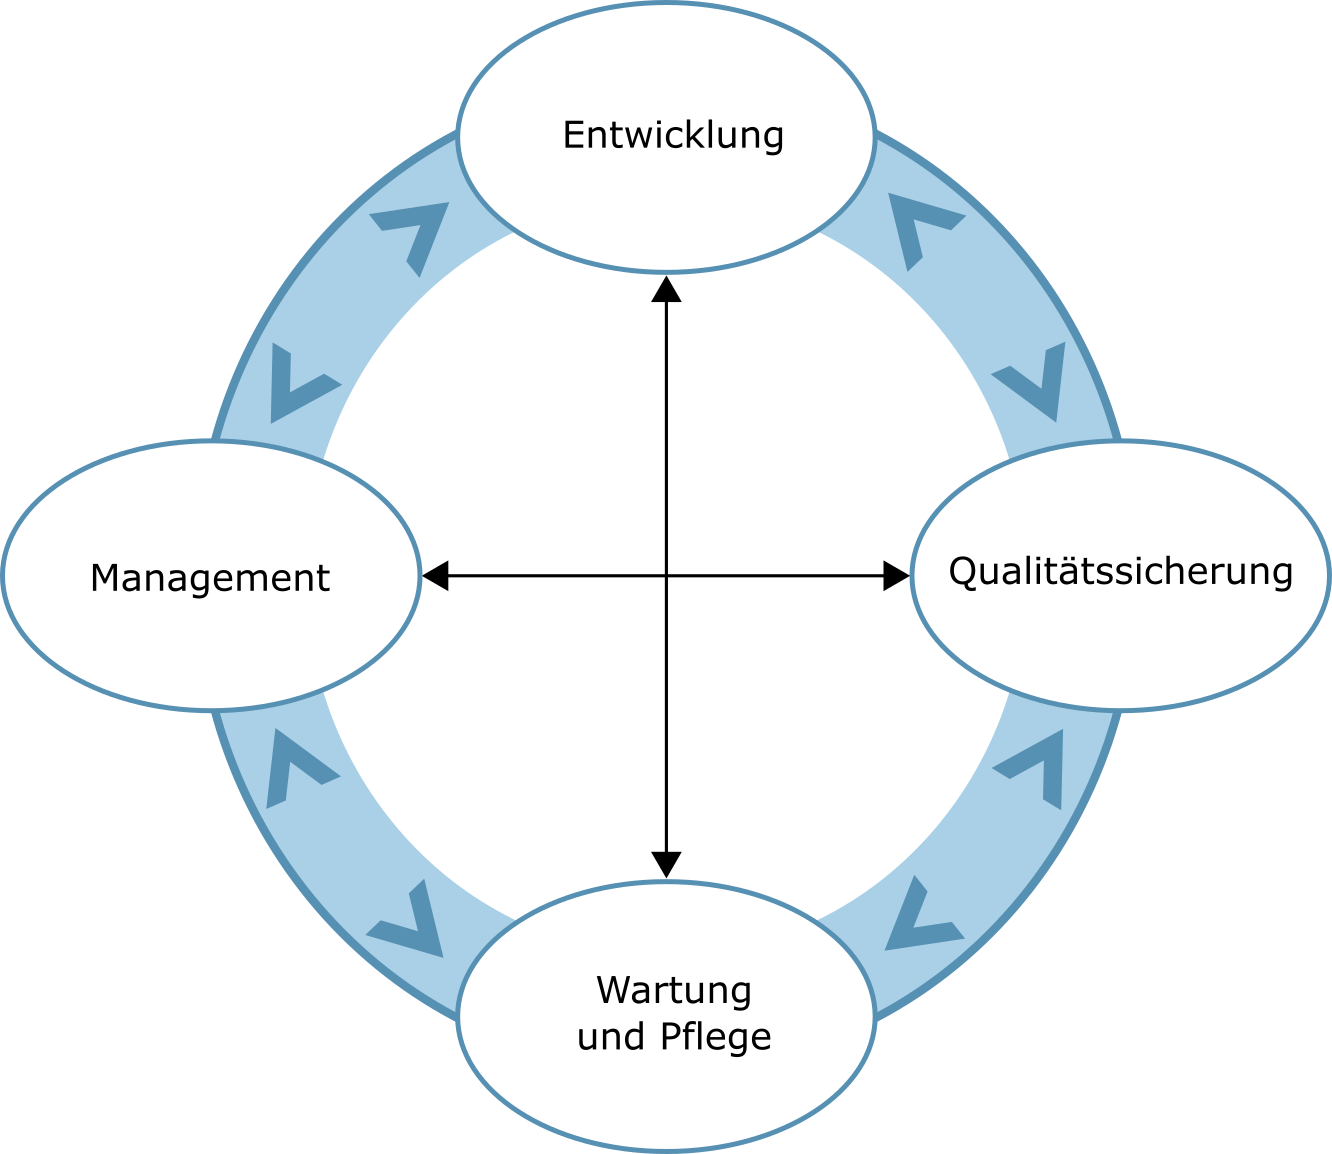
\includegraphics[width=0.5\textwidth]{./images/AbbEntwicklgProzess.png}
  \captionsetup{name=Abb.,font=footnotesize}
  \caption{Phasen im Software-Entwicklungsprozess (zyklischer Ansatz)}
\end{figure}
\newpage


\textbf{Entwicklung}
\newline
Die Software-Entwicklung hat die Aufgabe ein Produkt zu erstellen, das die geforderten Qualit"atseigenschaften besitzt. Der Entwicklungsprozess wird im Allgemeinen in eine Reihe von Aktivit"aten aufgeteilt, deren Ergebnisse einzelne Teilprodukte sind. Solche Aktivit"aten werden nach zeitlichen, begrifflichen, technischen und/oder organisatorischen Kriterien zu Phasen zusammengefasst.
\smallbreak
\textbf{Management}
\newline
Das Software-Management ist erforderlich, um den Entwicklungsprozess zu \textbf{planen}, zu \textbf{organisieren}, zu \textbf{leiten} und zu \textbf{kontrollieren}. Entwicklung und Management im Software-Entwicklungsprozess sind vielfach voneinander abh"angig. Die Einf"uhrung ne"ur Methoden und Tools kann zu Ver"anderungen in den organisatorischen Strukturen f"uhren.
\smallbreak
\textbf{Qualit"atssicherung}
\newline
Die Sicherstellung einer geforderten Softwarequalit"at muss durch eine entwicklungsbegleitende Software-Qualit"atssicherung erreicht werden. Dazu sind eine Reihe von konstruktiven und analytischen Ma"ssnahmen durchzuf"uhren. Die Ma"ssnahmen der Qualit"atssicherung werden dabei sowohl von der Entwicklung (die verwendeten Methoden, Tools und Programmiersprachen erfordern bestimmte Sicherungs- und Pr"ufma"ssnahmen), als auch vom Management durch organisatorische Zuordnung der Qualit"atssicherung zum Entwicklungsprozess beeinflusst.
\smallbreak
\textbf{Wartung und Pflege}
\newline
Nachdem ein Softwareprodukt zur Anwendung freigegeben wurde, beginnt die Wartung und Pflege, d. h. es gilt alle nach Inbetriebnahme auftretenden Fehler zu beseitigen, das Anwendungssystem an ver"anderte Bedingungen anzupassen und es bei Vorliegen ne"ur Anforderungen weiterz"untwickeln. Art und Umfang der Wartungst"atigkeiten sind auch von der Gew"ahrleistung der Qualit"atssicherung abh"angig, d. h. eine schlechte Produktqualit"at f"uhrt zwangsl"aufig zu h"aufigeren Fehleranteilen.

%-------------------------------------------------------------------------------
% Phasen der Entwicklung (wasserfallartig)
%-------------------------------------------------------------------------------
\newpage
\begin{figure}[H]
  \centering
  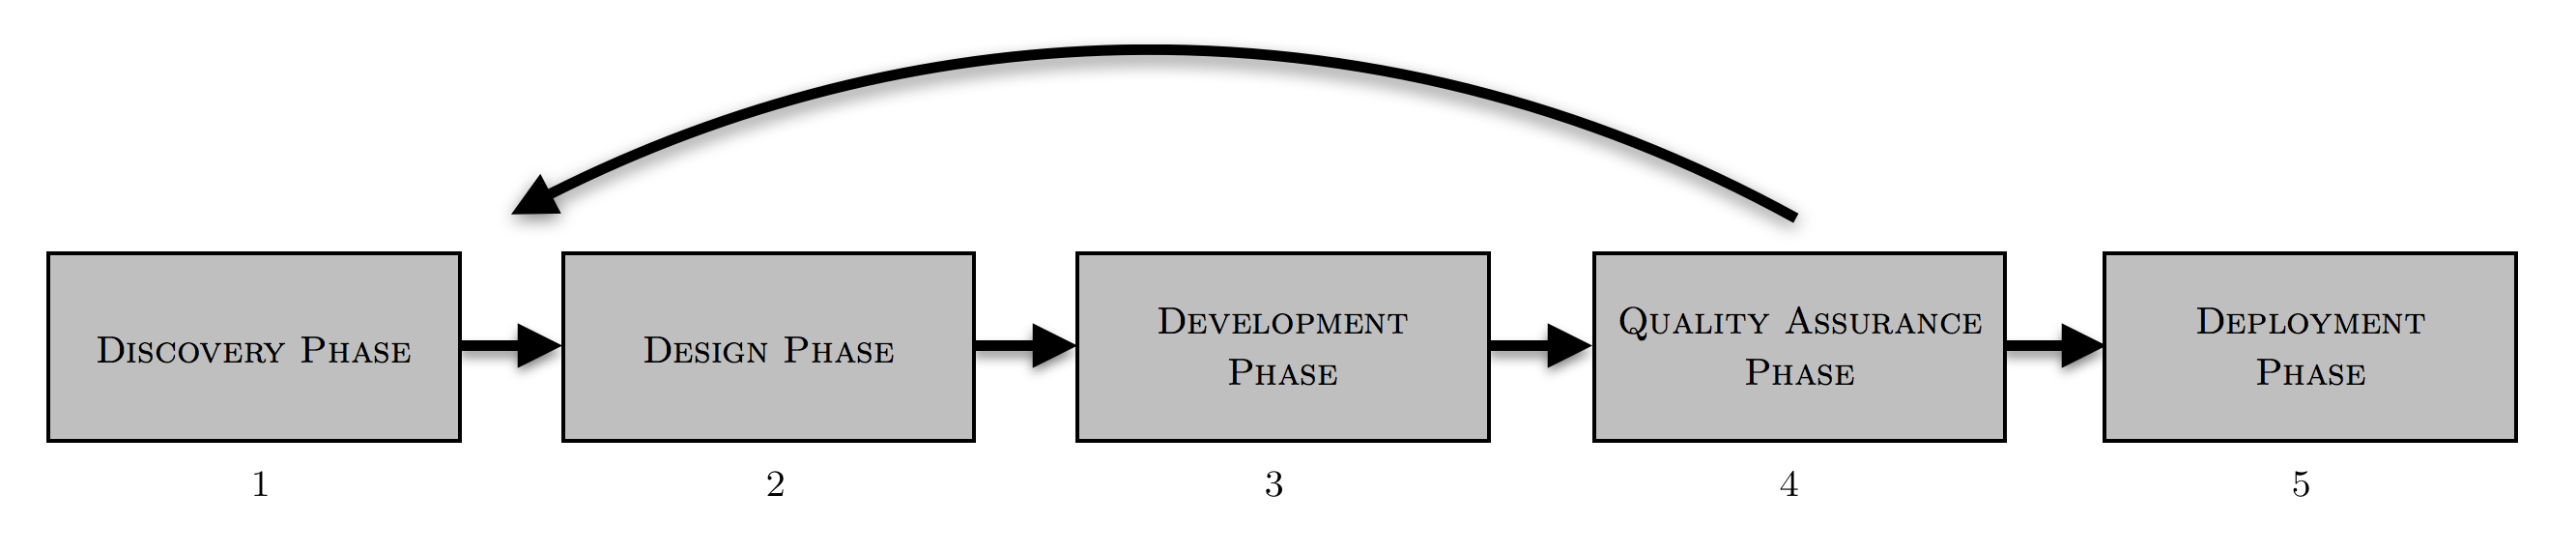
\includegraphics[width=1\textwidth]{./images/Softwarezyklus.png}
  \captionsetup{name=Abb.,font=footnotesize}
  \caption{Phasen im Software-Entwicklungsprozess (wasserfallartiger Ansatz)}
\end{figure}

\underline{\textbf{1. Discovery Phase:}}
\smallbreak
Diese Phase beinhaltet laut Balzert(1998)\supercite{Balzert1998} die \textbf{Analyse-} und \textbf{Definitionsphase}.
In der \textbf{Analysephase} wird die Ausgangssituation beschrieben,
die Ziele definiert und der daraus resultierende Ressourcenaufwand (\enquote{Scope of Work}) eruiert.\smallbreak
Diese Phase l"asst sich in folgende Aktivit"aten unterteilen:
\begin{itemize}
\item in eine Voruntersuchung (Marktanalyse, Trends, Kundenanfragen - \enquote{Idea Dump}),
\item eine Erhebung der Ist-Situation,
\item eine Erstellung einer Uebersicht der Bestandteile (\enquote{Information Architecture}),
\item eine Durchf"uhrbarkeitsuntersuchung (\enquote{Proof of Concept})
\end{itemize}
Diese m"unden in einem Projektplan und einer aus der Wirtschaftlichkeitsbetrachtung ergebenden Projektkalkulation.
\smallbreak
In der \textbf{Definitionsphase} werden die Anforderungen an das geplante Softwaresystem aus Anwendersicht und Pr"amissen f"ur die Realisierung des Softwaresystems definiert.\smallbreak
Diese Phase l"asst sich in folgende Aktivit"aten unterteilen:
\begin{itemize}
\item Ermittlung der Anforderungen
\item Beschreibung und Festlegung der Anforderungen
\item Validierung der Anforderung auf Konsistenz, Vollst"andigkeit und technische Durchf"uhrbarkeit
\end{itemize}

Diese Aktivit"aten resultieren in einem Daten- bzw. Funktionsmodell samt Benutzerschnittstelle und Projektplan und der sich darausergebenden Produktdefinition.

\bigbreak
\underline{\textbf{2. Design Phase:}}
\smallbreak
Diese Phase beinhaltet laut Balzert(1998)\supercite{Balzert1998} die \textbf{Entwurfsphase}.

In der \textbf{Entwurfsphase} wird ein softwaretechnischer Entwurf erarbeitet und beinhaltet folgende Aktivit"aten:
\begin{itemize}
  \item Analyse der Einsatzbedingungen sowie der Umgebungs- und Randbedingungen
  \item Definition der Systemkomponenten
  \item Entwurf der Systemarchitektur (Komponenten, deren Zusammenwirken und Anordnung)
  \item Entwurf der Schnittstellen und Festlegen ihrer Wechselwirkungen
  \item Validierung der Systemarchitektur
\end{itemize}
Sie m"undet in einer Beschreibung der Struktur des Software-Entwurfs und der Systemkomponenten.

\bigbreak
\underline{\textbf{3. Development Phase:}}
\smallbreak
Diese Phase beinhaltet laut Balzert(1998)\supercite{Balzert1998} die \textbf{Implementierungsphase}.

In der \textbf{Implementierungsphase} wird die Umsetzung der Entwurfsergebnisse in eine ausf"uhrbare Form "uberf"uhrt und eine Sicherung der Richtigkeit und Fehlerfreiheit der Ergebnisse der Systemimplementierung gew"ahrleistet.

Sie beinhaltet folgende Aktivit"aten:
\begin{itemize}
  \item Verfeinerung der Algorithmen f"ur die einzelnen Systemkomponenten
  \item Kodierung / Generierung der Algorithmen
  \item "Uberf"uhrung des logischen Datenmodells in ein physisches DB-Konzept
  \item Pr"ufung der semantischen Richtigkeit der Systemkomponenten
  \item Test der Syntax und gegebenenfalls Korrektur der fehlerhaften Systemkomponenten
  \item Pr"ufung des Zusammenwirkens der Systemkomponenten unter realen Bedingungen
  \item Feststellen und Beseitigen der Fehler im Softwaresystem
\end{itemize}
Sie m"undet in einer Bereitstellung der Q"ulltexte f"ur die Systemkomponenten, der Protokolle der Komponententests und Systemtests und generierten Datenobjekten und Datenstrukturen.
\bigbreak
\underline{\textbf{4. Quality-Assurance Phase:}}
\smallbreak
Diese Phase beinhaltet laut Balzert(1998)\supercite{Balzert1998} die \textbf{Abnahme-/ Einf"uhrungsphase}.

In der \textbf{Abnahme-/ Einf"uhrungsphase} Abnahme des fertiggestellten Softwareproduktes und Einf"uhrung beim Anwender realisiert.

Sie beinhaltet folgende Aktivit"aten:

\begin{itemize}
  \item "Ubergabe des Softwareproduktes einschlie"sslich Dokumentation an den Auftraggeber
  \item Durchf"uhrung eines Abnahmetests
  \item Installation des Softwareproduktes in dessen Zielumgebung
  \item Schulungen der sp"ateren Benutzer der Software
  \item Inbetriebnahme des Produktes
\end{itemize}

Sie m"undet im Erfolgsfall in ein gut dokumentiertes "ubergebenes Softwareprodukt.
\bigbreak
\underline{\textbf{5. Deployment Phase:}}
\smallbreak

Diese Phase beinhaltet laut Balzert(1998)\supercite{Balzert1998} die \textbf{Wartungs-} und \textbf{Pflegephase}.

In dieser Phase beinhaltet die Gew"ahrleistung der produktiven Nutzung des Anwendungssystems, Fehlerbeseitigung am Softwaresystem in der Betriebs- bzw. Nutzungsphase und die Realisierung notwendiger "Anderungs- und Erarbeitungsarbeiten.

Sie beinhaltet folgende Aktivit"aten:
\begin{itemize}
  \item Wartung: Stabilisierung und Optimierung der Produktinstallation
  \item Pflege: Anpassungen und Erweiterungen
\end{itemize}

Sie endet mit der Auslieferung und der Wartung der Software und resultiertert in einer maximalen Kundenzufriedenheit.
\begin{figure}[H]
  \centering
  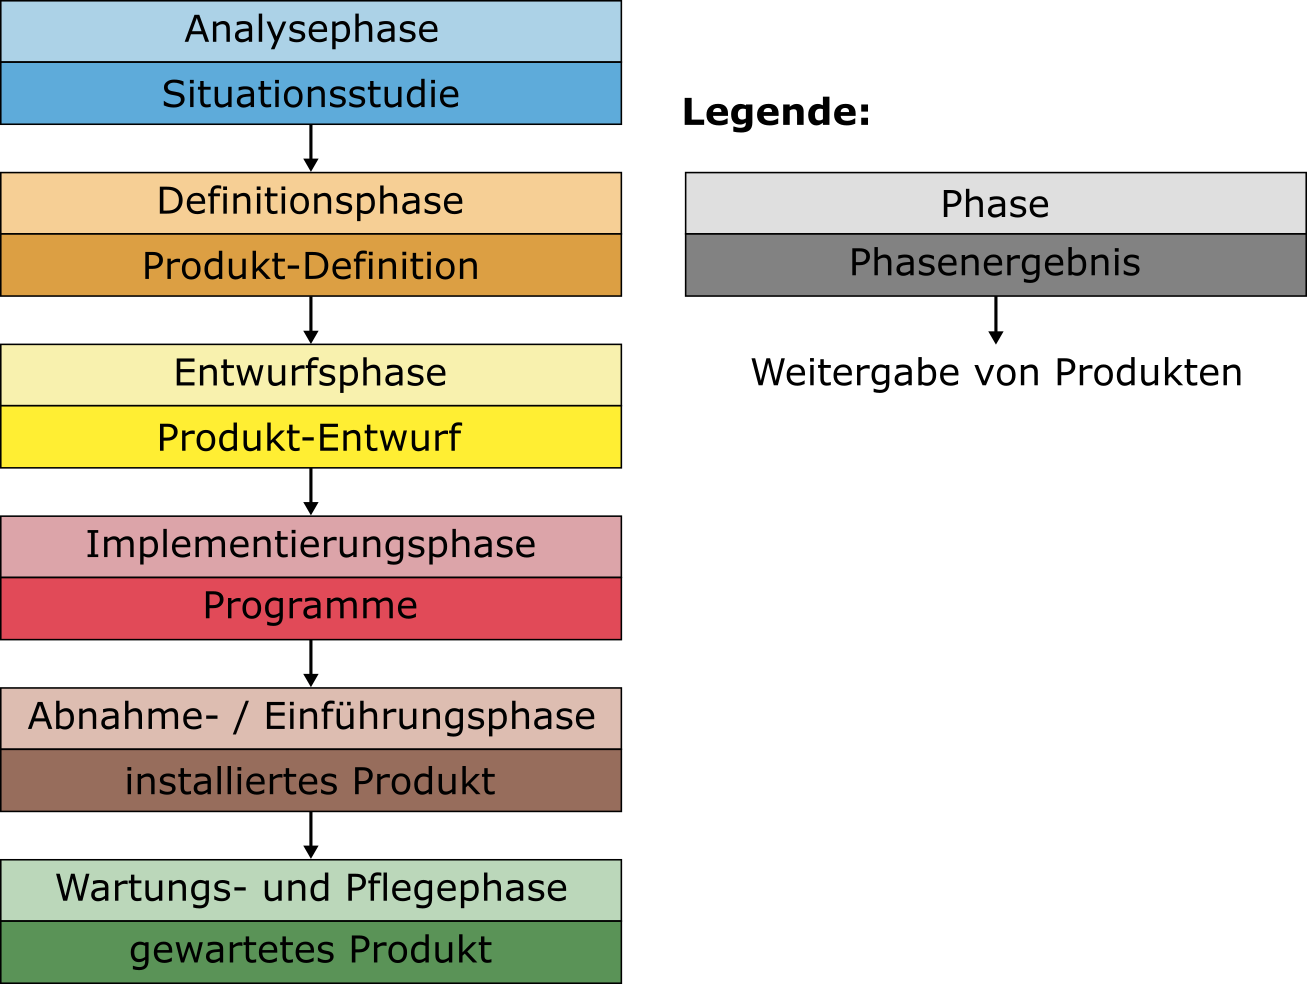
\includegraphics[width=0.8\textwidth]{./images/AbbPhaseneinteilung.png}
  \captionsetup{name=Abb.,font=footnotesize}
  \caption{Phaseneinteilung (wasserfallartig) nach Balzert(1998)\supercite{Balzert1998}}
\end{figure}


%-------------------------------------------------------------------------------
% #3
%-------------------------------------------------------------------------------
\newpage
\subsection{"Ubung SWT-03}
\subsubsection*{Aufgabe:}

\begin{framed}
\textbf{Prinzipien}
\smallbreak
Geben Sie bitte zu jedem Prinzip der Softwaretechnik (Abstraktion, Strukturierung, Hierarchisierung, Modularisierung, Standardisierung) ein Beispiel an. Wo ist Ihnen das schon begegnet und wo k"onnte das in der Softwaretechnik angewendet oder wirksam werden?
\bigbreak
\small Bearbeitungszeit: 10 Minuten
\end{framed}
\bigbreak
\bigbreak
\subsubsection*{L"osung:}
\textbf{Abstraktion}
- Beispiel: Authentifizierungslogik einer Applikation
\smallbreak
Angenommen es gibt in einer Applikation verschiedene Sichtweise auf eine Applikation.
\smallbreak
Zum Beispiel eine normale User-Sicht welche in ihren Rechten beschr"ankt ist und es dadurch eingeschr"ankte Nutzungsm"oglichkeiten gibt.
Gerade bei der Entwicklung einer ACL bzw einer Rollenbasierten Authentifizierung innerhalb einer Applikation benutzt man Abstraktion um nicht alle Rechte/Rollen und deren Konsequenzen bis ins Detail zu konkretisieren, sondern ein abstraktes Modell der Rechte zu entwickeln.
Man spricht dabei zum Beispiel von einem User-Kontext und einen Administrativen-Kontext.

In Bezugnahme zu sogenannten CRUD Anwendungen sind in dem User Kontext nur lesende Zugriffe auf das Inhaltsmodell m"oglich , wohingegen in dem Administrativen Kontext ein Vollzugriff m"oglich ist.

Der Komplexit"atsgrad steigt mit dem Funktionsumfang, wenn man zum Beispiel dem User erlaubt eigene Crud Inhalte in vollem Umfang zu verwalten - so muss man das Inhaltsmodell an das Usermodell binden.
Um die Komplexit"at in diesem Fall einzugrenzen bedient man sich zum Beispiel der klassenbildenden Abstraktion. Man abstrahiert den Sachverhalt auf gemeinsame Merkmale (im obigen Beispiel das R - Read) und bildet spezielle Merkmale (C - Create , U - Update und D - Delete).

Im obigen Beispiel wird die Inhaltsmenge die man aus dem User-Kontext konsumieren kann als Teilmenge der aus dem Administrativen-Kontext gegebenen Inhaltsmenge angesehen.
Man konkretisiert diese Inhaltsmenge nicht sondern abstrahiert nur deren Authentifizierung darauf. Durch Abstraktion ist es m"oglich das komplexe Problem Authentifizierung auf verschiedene Ebenen zu verteilen. Diese Trennung wird durch das Erfassen des Wesentlichen und das Weglassen von Besonderem realisiert.



\textbf{Strukturierung}
- Beispiel: Architektur einer Webapplikation (MVC Pattern)

Das Prinzip der Strukturierung kann man am Beispiel des Architektur Patterns MVC sehr gut erkl"aren.
Es strukturiert eine Applikation durch die Trennung des Inhalt (Business Logik - Controller) vom Design (das Frontend - Design).
Es hat den Vorteil das das Frontend unabh"angig (parallel) vom Entwicklungsstand der Applikation entwickelt werden kann - das Prinzip hat eine grosse Bedeutung f"ur den Entwicklungsprozess einer Applikation.

Mithilfe von Development-Seeds bzw. Dummy Data ist es dem Frontend Entwickler m"oglich abgetrennt von der Business Logik zu entwickeln - es stellt somit eine elementare Basis f"ur die Arbeitsteilung dar.

Dar"uberhinaus hilft es bei der Bew"altigung der Komplexit"at und f"uhrt zu einer erh"ohten Verst"andlichkeit f"ur Produkt und Prozess.

Durch Abtrennung dieser Dom"anen erh"oht es zu dem die Wartbarkeit und die Einarbeitung in ein fremdes Softwareprodukt (reverse engineering).

Als Beispiel k"onnte man den klassisches Entwicklungsprozess einer Webapplikation anf"uhren. Es wird unabh"angig vom Controller die View entwickelt.
Die View (Frontend) kann auch erstmal mit hardcodierten Inhalten entwickelt werden und sp"ater mittels Templating mit produktiven Daten gef"ullt werden.

Oft kommen die produktiven Daten aus diversen Subsystemen (Backend) die f"ur einzelne Entwickler nicht allumfassend "uberschaubar sind.
Das Frontend muss sich also bei guter Gesamtstrukturierung nicht um die Richtigkeit/Validit"at der Daten k"ummern und kann sich voll und ganz auf die View's konzentrieren , ist also nicht verantwortlich f"ur die Datengenerierung sondern nur f"ur die Darstellung.

Ein weiteres Beispiel f"ur Strukturierung ist das Prinzip der Partials in einem Applikationsfrontend. Durch Partials ist es m"oglich ein Problem nur einmal zu definieren/auszuprogrammieren und entspricht dem DRY Best-Practise der Softwaretechnik.

\textbf{Hierarchisierung}

Das Prinzip der Hierarchisierung ist ein Spezialfall der Strukturisierung und bezeichnet eine Rangordung.

Als Beispiel kann man das Prinzip der Partials noch einmal aufgreifen. Dort wird eine Struktur der Applikation ausgehend von einem Main/Layout Partial hierrarchisch realisiert.
Die Applikation wird in Sektionen strukturiert. Es werden also bestimmte Sektionen in den Code injeziert (yielding).

Es ist also m"oglich eine Applikation in Hauptseiten und Unterseiten bzgl. der Hierarchie zu strukturieren.
Das Prinzip der Hierarchie liegt eine Baumstruktur - in diesem Fall als Wurzel das Mainpartial - zu grunde.

\newpage
\textbf{Modularisierung}

In jedem Oekosystem einer Programmiersprache hat man M"oglichkeiten auf Module zur"uckzugreifen und bestimmte Probleme nicht noch einmal l"osen zu m"ussen. (Ueber dieverse Packagemanager (npm, gems, composer, maven/ant, pip etc.))

Ein Modul bietet die M"oglichkeit der Aufgliederung eines Softwaresystems in diverse Subsysteme. Das hat den Vorteil das die Komplexit"at durch das Prinzip ``divide and conquer'' geb"andigt wird.
Diese Module bieten diverse Schnittstellen f"ur den In/Output und sind in sich abgeschlossen und wiederverwendbar.

Dar"uberhinaus sind Module in sich wartbar (vom Maintainer) und abgekapselt vom Hauptsystem.

Ich hatte zum Beispiel in Java das Problem der Serialization/Deserialization von JSON.
Nat"urlich h"atte ich auch das Rad neu erfinden k"onnen und es mit den Werkzeugen der Programmiersprache selbst l"osen k"onnen.
Viel einfacher ging das aber "uber ein Modul von Google GSON was eine Abstraktionsebene dazwischen geschalten hat und letztlich schneller zum Erfolg f"uhrte.

Oder die Authentifizierung gegen"uber eines LDAP dort habe ich auf ein composer package ADLAP2 zur"uckgegriffen was genau das tut was ich m"ochte. Ich musste nicht verstehen wie es die Authentifizierung gegen"uber einen LDAP genau macht - ich musste nur verstehen es anzuwenden.

Als Anlaufstelle f"ur diverse Packages Module in diversen Sprachen nutze ich immer wieder Github - weil dort 99\% aller meiner Probleme schon gel"ost sind und ich mich der eigentlich Problematik meines Systems widmen kann.

Es geht mittlerweile soweit das ich an diversen stelle schon Contribute weil ich Nutzungsszenarien entdecke die so vom Modul noch nicht bedacht sind.

Problematisch sehe ich jedoch das ich durch die Nutzung von Fremdmodulen mich in eine Abh"angigkeit des Packages/Modules begebe. Oft werden diverse Packages umgebaut (die schnittstellen ver"andert) das ein Upgrade so nicht einfach m"oglich ist.
Dar"uberhinaus sehe ich es als problematisch an gerade bei sensiblen funktionen (authentifizierung einer applikation) nicht nur auf die funktionalit"at eines moduls zu vertrauen sondern viel mehr auf die kompetenz des entwickelnden.
Dem gegen"uber steht die Open-Source Bewegung wo jeder Code Review betreiben kann und Issues tracken kann und Contributen kann.

Ein schoenes Paper zu der Problematik:
https://arxiv.org/pdf/1704.02786.pdf



\textbf{Standardisierung}

Das Prinzip der Standardisierung beinhaltet die Vereinheitlichung des Entwicklungsprozesses und des Produktes. Der wichtigste Aspekt ist die Kostenminifizierung. Der Aufwand wird gemindert durch das Einf"uhren von Standards.
Es entwickelte sich dazu das Paradigma ``Convention over Configuration'', was die Konvention vor die Konfiguration stellt und so den Konfigurationsaufwand mindert. (siehe Ruby on Rails)

Ich erlebe in meiner berfulichen Welt st"andig Standards mit denen ich konfrontiert werde.
Angefangen bei ganz banalen Sachen wie die Camel-Case Notation in der Namensgebung von Variablen/Methoden/Klassen.
Aber auch die Namensgebung bestimmter Branches (Feature Branches) inklusive Issue Nummer.

Ich denke das Standards die Qualit"at der Zuarbeit immens erh"ohen k"onnen.
Das f"angt beim einrichten der Entwicklungsumgebung an so das wir bei XP (Pairprogramming) eine Dev-Environment haben wo wir uns schnell einarbeiten und produktiv werden, "uber die Namensgebung bis hin zu den Zusammenfassen von Commits bei einem MergeRequest im GIT.

Alles unter dem Aspekt ein Enhancement zu haben bzgl. des kollaborativen Arbeitens.


%-------------------------------------------------------------------------------
% #4
%-------------------------------------------------------------------------------
\newpage
\subsection{"Ubung SWT-04}
\subsubsection*{Aufgabe:}

\begin{framed}
\textbf{Recherche}
\smallbreak
Recherchieren Sie bitte im Internet "uber Softwaretechnik oder Softwareengineering. Welche Bereiche interessieren Sie ganz besonders?
\bigbreak
\small Bearbeitungszeit: 30 Minuten
\end{framed}
\bigbreak
\bigbreak
\subsubsection*{L"osung:}
Lorem ipsum dolor sit amet, consectetur adipisicing elit, sed do eiusmod tempor incididunt ut labore et dolore magna aliqua. Ut enim ad minim veniam, quis nostrud exercitation ullamco laboris nisi ut aliquip ex ea commodo consequat. Duis aute irure dolor in reprehenderit in voluptate velit esse cillum dolore eu fugiat nulla pariatur. Excepteur sint occ"acat cupidatat non proident, sunt in culpa qui officia deserunt mollit anim id est laborum.

%-------------------------------------------------------------------------------
% #5
%-------------------------------------------------------------------------------
\newpage
\subsection{"Ubung SWT-05}
\subsubsection*{Aufgabe:}

\begin{framed}
\textbf{Wissensfragen zur Lerneinheit}
\smallbreak
Versuchen Sie die Fragen schriftlich zu beantworten ohne noch einmal in der Lerneinheit nachzuschlagen.
\begin{enumerate}
\item An welche Best Practices erinnern Sie sich oder welche haben Sie verinnerlicht?
\item Warum ist es sinnvoll Softwarefehler fr"uh zu erkennen?
\item Was geht in Softwareprojekten typischerweise schief?
\item Kennen Sie (Standardisierungs-)Organisationen, die sich mit Software besch"aftigen?
\end{enumerate}
\bigbreak
\small Bearbeitungszeit: 15 Minuten
\end{framed}
\bigbreak
\bigbreak
\subsubsection*{L"osung:}
Lorem ipsum dolor sit amet, consectetur adipisicing elit, sed do eiusmod tempor incididunt ut labore et dolore magna aliqua. Ut enim ad minim veniam, quis nostrud exercitation ullamco laboris nisi ut aliquip ex ea commodo consequat. Duis aute irure dolor in reprehenderit in voluptate velit esse cillum dolore eu fugiat nulla pariatur. Excepteur sint occ"acat cupidatat non proident, sunt in culpa qui officia deserunt mollit anim id est laborum.

%-------------------------------------------------------------------------------
% #6
%-------------------------------------------------------------------------------
\newpage
\subsection{"Ubung SWT-06}
\subsubsection*{Aufgabe:}

\begin{framed}
\textbf{Fehlerquellen}
\smallbreak
H"aufige Fehlerq"ullen in Softwareprojekten sind:
\bigbreak
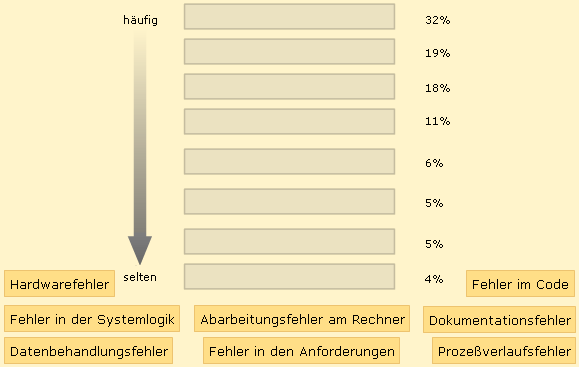
\includegraphics[width=1.0\textwidth]{./images/ueb01-06.png}
\end{framed}
\bigbreak
\bigbreak
\subsubsection*{L"osung:}
Lorem ipsum dolor sit amet, consectetur adipisicing elit, sed do eiusmod tempor incididunt ut labore et dolore magna aliqua. Ut enim ad minim veniam, quis nostrud exercitation ullamco laboris nisi ut aliquip ex ea commodo consequat. Duis aute irure dolor in reprehenderit in voluptate velit esse cillum dolore eu fugiat nulla pariatur. Excepteur sint occ"acat cupidatat non proident, sunt in culpa qui officia deserunt mollit anim id est laborum.

%-------------------------------------------------------------------------------
% #7
%-------------------------------------------------------------------------------
\newpage
\subsection{"Ubung SWT-07}
\subsubsection*{Aufgabe:}

\begin{framed}
\textbf{Phaseneinteilung}
\smallbreak
Ordnen Sie die Phasen und Ergebnisse des Softwarelebenszyklus in der richtigen Reihenfolge an.
\bigbreak
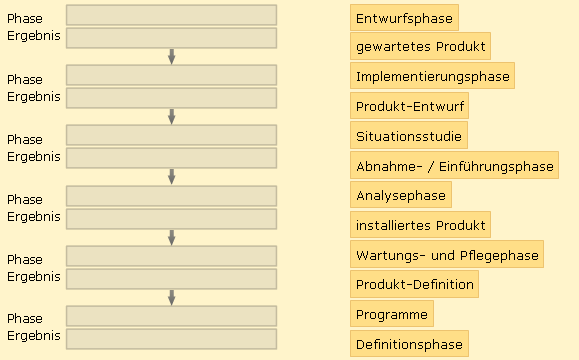
\includegraphics[width=1.0\textwidth]{./images/ueb01-07.png}
\end{framed}
\bigbreak
\bigbreak
\subsubsection*{L"osung:}
Lorem ipsum dolor sit amet, consectetur adipisicing elit, sed do eiusmod tempor incididunt ut labore et dolore magna aliqua. Ut enim ad minim veniam, quis nostrud exercitation ullamco laboris nisi ut aliquip ex ea commodo consequat. Duis aute irure dolor in reprehenderit in voluptate velit esse cillum dolore eu fugiat nulla pariatur. Excepteur sint occ"acat cupidatat non proident, sunt in culpa qui officia deserunt mollit anim id est laborum.









%-------------------------------------------------------------------------------
% Literatur - Glossar - Akronyme
%-------------------------------------------------------------------------------

\clearpage
\setlength\bibitemsep{10pt}
\printbibliography[heading=bibintoc]
\newpage
\printglossary[type=main]
\printglossary[type=\acronymtype]


%-------------------------------------------------------------------------------
% ENDE
%-------------------------------------------------------------------------------

\end{document}
